% Please make sure you insert your
% data according to the instructions in PoSauthmanual.pdf

\documentclass[a4paper]{PoS}
\usepackage{color}
\usepackage{graphicx}
\usepackage{caption}
\usepackage{subcaption}
%\usepackage{apacite}
\usepackage{lineno}
\linenumbers



\title{Development and testing of a Trigger Processor Card based on a Kintex Ultrascale FPGA.}

\ShortTitle{Development of a Trigger Processor Card based on a Kintex Ultrascale FPGA.}



\author{\speaker{S. Mallios}\textsuperscript{ a}, K. Adamidis\textsuperscript{a}, G. Bestintzanos\textsuperscript{a}, C. Fountas\textsuperscript{a}, G. Karathanasis\textsuperscript{c}, P. Katsoulis\textsuperscript{a}, N. Manthos\textsuperscript{a}, I. Papadopoulos\textsuperscript{a}, S. Sotiropoulos\textsuperscript{b}, P. Sphicas\textsuperscript{c}, C. Vellidis\textsuperscript{c}\\
\llap a) University of Ioannina, Greece\\
\llap b) Institute of Accelerating Systems and Applications (IASA), Athens, Greece\\
\llap c) University of Athens, Greece\\
E-mail: \email{stavros.mallios@cern.ch}}



%University of Ioannina1, University of Athens2 and Institute of Accelerating Systems and Applications (IASA), Athens3


\abstract{During the HL-LHC era, the upgraded detector will be read-out at an unprecedented event rate of 750~KHz and a data rate of up to 50~Tb/s. Within the context of Phase-2 R\&D, a Level-1 Trigger processor card was designed, by the Greek CMS Trigger team, to provide a hardware environment for developing and evaluating new Level-1 trigger muon designs and technologies. The board is powered by the XCKU040 Kintex UltraScale FPGA. A new firmware was also developed implementing 16~Gbps links with IPbus support, for testing new algorithms. The hardware and firmware design of the board is presented.}


\FullConference{Topical Workshop on Electronics for Particle Physics (TWEPP2018)\\
		17-21 September 2018\\
		Antwerp, Belgium}





\begin{document}

\pagenumbering{arabic}


\section{Introduction}
The upgraded High Luminosity LHC, after the third Long Shutdown (LS3), will provide an instantaneous luminosity of $7.5 \times 10^{34} cm^{-2} s^{-1}$ (levelled), at the price of a dramatic increase of the number of pileup interactions. It is expected that the number of pileup interactions could reach 200 per bunch crossing. The upgraded detector will be read-out at an unprecedented event rate of 750~KHz and a data rate of up to 50 Tb/s \cite{Collaboration:2283192}. Within the scope of Phase 2 R\&D, a new Level-1 Trigger processor card was designed, by the CMS Trigger teams from the University of Athens and the University of Ioannina, to provide a hardware environment for developing and evaluating new Level-1 trigger muon designs and technologies. The board comes with state-of-the-art fiber optics technologies, using micro footprint optical interconnects. For testing purposes, a new firmware was developed, implementing asynchronous 16~Gbps GTH links. The links use the 64b/66b encoding scheme with an overhead of 2 coding bits per 64 bits that is considerably more efficient than the 8b/10b encoding scheme. The hardware and firmware design of the processor card is presented.

\section{The hardware}
The board is powered by the XCKU040 Kintex UltraScale FPGA, providing 20 next-generation GTH transceivers, that reach speeds up to 16.3~Gbps. The board comes with state-of-the-art fiber optics technologies from Samtec. The high performance interconnect system uses active optical engines over 12 full-duplex channels, at data rates up to 16~Gbps. Furthermore, 4 FPGA transceivers are routed to a QSFP28 connector, which can handle data rates of up to 28~Gbps per channel over 4 channels. In total, the board's 16x16 Gbps links, add up to a total optical bandwidth of approximately 256~Gbps in each direction, making it a high-performance all-optical data-stream processor (Figure \ref{fig1}). A Xilinx ZYNQ System-on-Chip (SoC) device will be used as the control interface for the Kintex UltraScale FPGA. The system controller sets up or queries on-board resources, such as the power controllers and programmable clocks.

\begin{figure}[h]
\centering
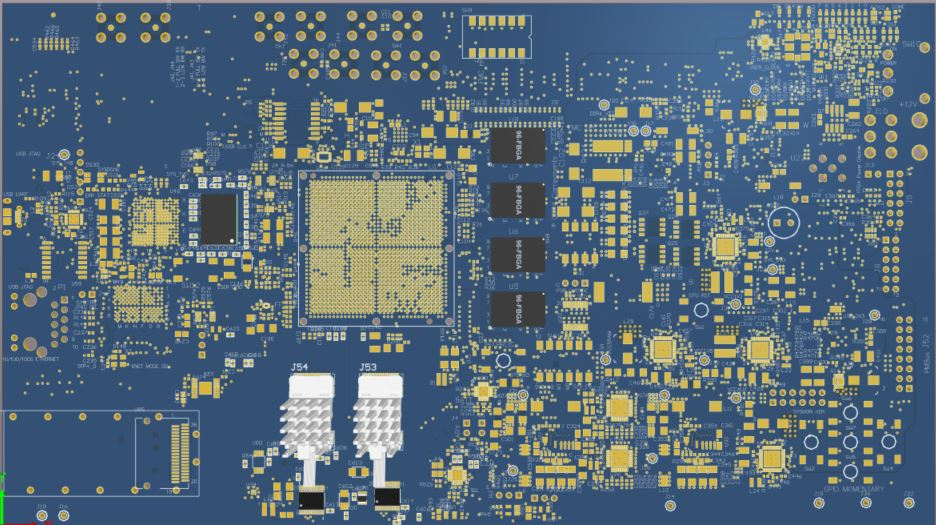
\includegraphics[width=0.8\textwidth]{board_3D_altium.png}
\caption{Altium 3D representation of the board}
\label{fig1}
\end{figure}



\subsection{The FPGA}
The onboard XCKU040 FPGA, a  mid-range Xilinx Kintex Ultrascale high-performance FPGA which focuses on a price/performance ratio. It has high DSP and block RAM-to-logic ratios and next-generation transceivers. Combined with low-cost packaging, it enables an optimum blend of capability and cost. The part is available in a FFVA1156 package, with all the high speed Multi-Gigabit Transceivers (MGTs)  placed on the left side of the part. The ultrascale architecture provides key innovations like next generation routing, ASIC-like clocking and enhanced logic blocks for a target of 90\% utilization high-speed memory cascading, to remove bottlenecks in DSP and packet processing \cite{mehta2013xilinx}.
The board also includes 2~GB of DDR4 memory (four [256~MB x 16] devices) at 1200~MHz / 2400~Mbps.

%\begin{figure}[h]
%\centering
%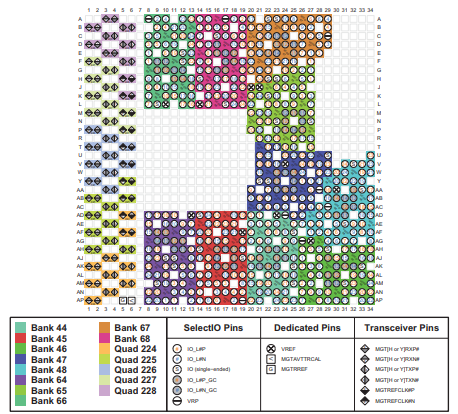
\includegraphics[width=0.8\textwidth]{xcku040_pinout.png}
%\caption{FFVA1156 Package - XCKU040 I/O Bank Diagram}
%\label{xcku040}
%\end{figure}


\subsection{High Speed Optical Links}
The data-interface consists of 16 optical links, operating in excess of 16 Gbps, making full use of the MGTs available on the Kintex Ultrascale FPGA. Twelve (12) of the optical links are routed to the FireFly optical flyover assembly (Figure \ref{firefly}), that is placed next to the FPGA \cite{zbinden2018connector}. The FireFly configuration consists of 12 separate transmitter (TX) and receiver (RX) optical modules, joined in a "Y" configuration and terminate to a single 24 fiber MPO connector. The connectors are placed mid-board and the data "fly" over the PCB, allowing easier routing. Four more MGTs are routed to a QSFP28 (Finisar FTLC9551REPM) transceiver module. This module has a hot-pluggable QSFP28 form factor and supports 103.1~Gbps of aggregate bit rate. However, the rate is limited by the MGT's maximum speed to 64~Gbps.

\begin{figure}
\centering
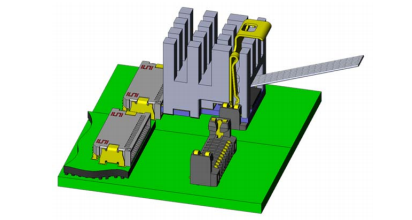
\includegraphics[width=0.6\textwidth]{firefly.png}
\caption{Miniature Patent Pending On-board Optical FireFly Micro
Flyover System (source: Samtec) }
\label{firefly}
\end{figure}


\subsection{Clocking}
The board includes 5 low-jitter programmable clock sources. The GTH transceivers connected to the high speed Firefly modules, are clocked by a dedicated, low jitter, quad clock generator (Si5338). A low-jitter frequency generator (Si570) is connected to the QSFP28 transceivers and can also be used as a secondary clock source to the Firefly transceivers. A jitter attenuator (Si5328B) is used to reduce the jitter of a received recovered clock. A fixed frequency clock source can be used as a free running clock for reset and initialization FSMs. Finally an SMA external clock input is also available. All programmable clocks are accessed through a dedicated I$^2$C bus.

%\begin{figure}[h]
%\centering
%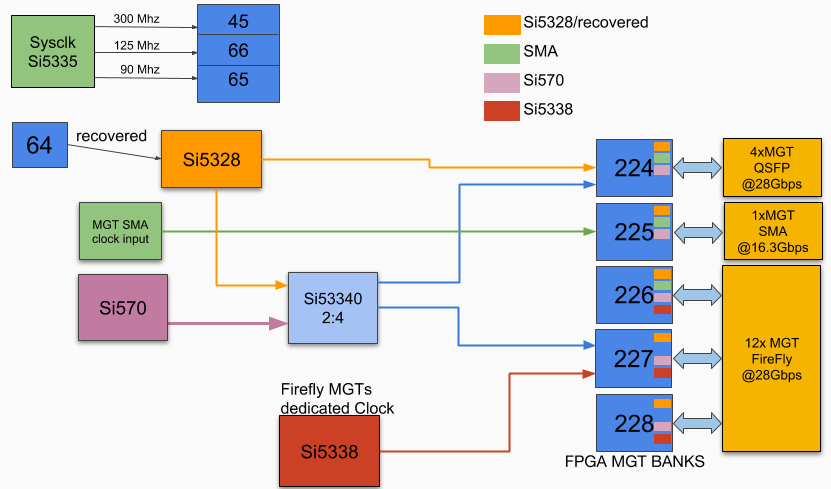
\includegraphics[width=0.8\textwidth]{clocking.png}
%\caption{ Clocking architecture of the board}
%\label{clocking}
%\end{figure}


\subsection{PCB}
The board provides 32 high speed differential-pairs running at 16~Gbps. The Firefly transceivers were placed very close to the FPGA's right side, achieving closer proximity to the Banks were all the MGTs reside, to simplify board layout and enhance signal integrity (Figure \ref{fig:toplayer}). For the substrate, the Panasonic Megtron-6 was chosen, due to the excellent high-frequency performance and impedance properties. A ground-plane has been placed between each layer containing high-speed traces, resulting in a 16-layer stack-up. All high speed differential pairs route lengths were matched by using serpentine routing (Figure \ref{fig:serpantine}). Finally, to avoid additional signal distortion caused by the plated-through hole (PTH) VIAs, we removed the excess via stub using a technique known as back-drilling.


\begin{figure}
\begin{subfigure}{.5\textwidth}
  \centering
  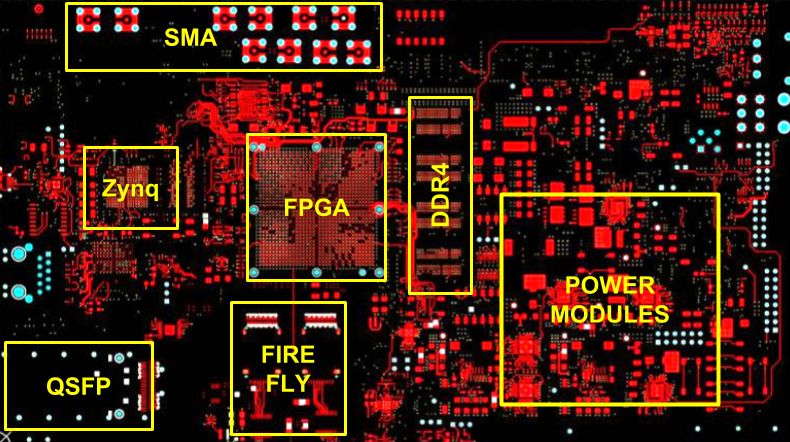
\includegraphics[width=1\linewidth]{pcb.png}
  \caption{PCB top layer}
  \label{fig:toplayer}
\end{subfigure}%
\begin{subfigure}{.5\textwidth}
  \centering
  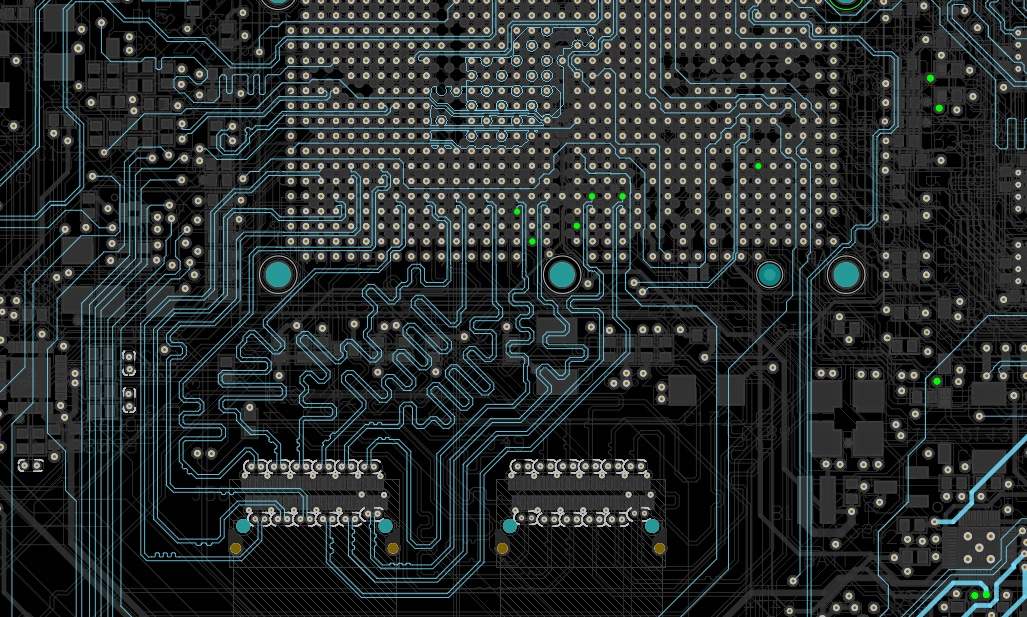
\includegraphics[width=0.9\linewidth]{serpentine_routing.png}
  \caption{Serpentine routing}
  \label{fig:serpantine}
\end{subfigure}
\caption{PCB details}
\label{fig:pcb}
\end{figure}



\section{Firmware}


\subsection{The protocol}
The 16~Gbps links firmware is a lightweight, link-layer protocol that can be used to move data point-to-point across one or more high-speed serial lanes. It supports simplex operation with continues data transfer. The links are asynchronous, meaning that the main algorithmic logic is clocked with a lower frequency than the link clock, allowing more flexibility when choosing the logic clock. This is achieved by using asynchronous FIFOs in the receiving and transmitting sides. To compensate for the difference of the frequency, padding words are being injected on the transmitting side and are stripped away on the receiving side. The link initialization and error handling are also based on the insertion and checking of those padding words. For testing purposes the local clock is running at 240 MHz and the link clock at 250 MHz. The link encoding is the 64b/66b encoding that transforms 64-bit data to 66-bit line code, to provide enough state changes to allow reasonable clock recovery and alignment of the data stream at the receiver \cite{walker200064b}. The protocol overhead of 64b/66b encoding is 2 coding bits for every 64 payload bits or 3.125\%. This makes the encoding considerably more efficient than the 25\% overhead of the previously-used 8b/10b encoding scheme, which added 2 coding bits to every 8 payload bits.



\subsection{Link initialization and error handling}
The link bring-up and error detection is based on the generic 2-bit 64b/66b encoding header, combined with the periodically sending of a padding word and CRC blocks. Single errors are considered soft errors and are monitored with a soft error counter. Continuous errors are considered hard errors and result in auto reset and re-alignment of the links. The overhead of the 64b/66b encoding is 3.125\% and the CRC/padding blocks are injected every 100 blocks resulting at a total overhead of 4.125\%. The maximum time for the link (re)alignment is 200 $\mu$s.

\begin{figure}
\centering
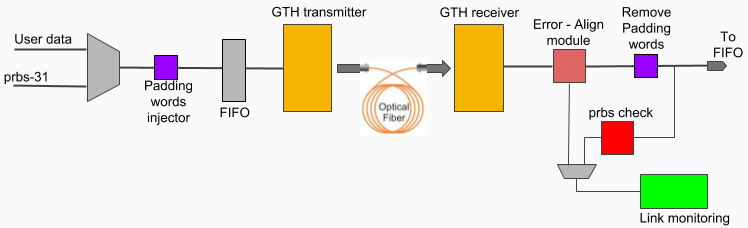
\includegraphics[width=1\textwidth]{link_align.png}
\caption{Link alignment and error handling block diagram}
\label{align}
\end{figure}


\subsection{Testing}
The functionality of the links was extensively tested using the KCU-105 Xilinx Ultrascale developement board. Bit Error Rate tests were performed, by sending PRBS-31 data over an FMC loopback card. The links operated for more than 72 hours without errors resulting in BER of less than $10^{-16}$. The latency of the GTH transceiver was reduced, by removing the internal elastic buffer, to 9 CLKs. The asynchronous FIFOs, however, add a latency of 6 CLKs on the transmittng side and 6 CLKs on the receiving end, adding up to a total link latency of 21 CLKs at 250~MHz.

 
\bibliography{test}
\bibliographystyle{JHEP}


\end{document}



